\toolname is a post-synthesis refinement layer for LLM-generated vulnerability detectors.  Given a draft CSA checker or CodeQL query produced by an upstream generator, the patch that motivated the synthesis, and the corresponding source tree and validation scope, \toolname refines the detector to encode missing semantic predicates while retaining a vulnerable-side warning signal.

% \subsection{Overview}

\begin{figure}[!htbp]
  \centering
  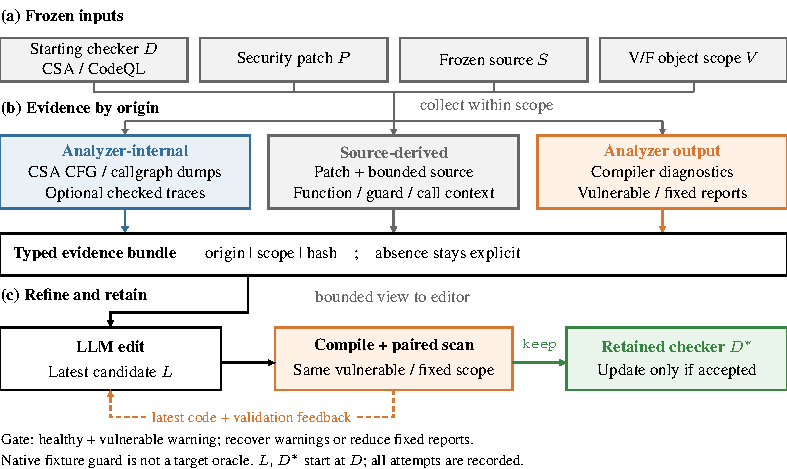
\includegraphics[width=\textwidth]{figures/fig-architecture-f258.pdf}
  \Description{Workflow from a generated checker and patch through evidence collection, a typed provenance-labelled bundle, checker editing, paired validation, and audit artifacts.}
  \caption{\textbf{\toolname architecture.}
  A generated detector, patch and bounded evidence feed the editor and paired retention rule. Native provenance is checked separately from collector names. Retention tracks version-warning presence, not target correctness; fixed silence is secondary. Inputs, rejected/retained candidates and raw validation records remain auditable.}
  \label{fig:approach-architecture}
\end{figure}

Figure~\ref{fig:approach-architecture} groups the workflow into three panels.
\textbf{(a)~Generator context.} The input is an existing detector, patch, source tree and validation scope, not a new generation task.
\textbf{(b)~Assembly and bundle.} Rule-guided preflight, source extraction, analyzer collection and validation feedback supply provenance-typed records and bounded views (Sections~\ref{sec:adaptive-selection}--\ref{sec:evidence-schema}).
\textbf{(c)~Paired-warning refinement.} The agent edits the latest attempted detector; normal paired outcomes update a separate best detector when they recover warning presence or reduce fixed reports while retaining it. Rejected attempts remain next-step input/feedback (Section~\ref{sec:refinement}).
\textbf{Audit artifacts.} The verifier checks raw-output/source-scope bindings, interfaces, provenance counts, selected code and paired logs. Original prompts, replies and all attempts persist; an LLM explanation is not an origin certificate.

\begin{algorithm}[t]
\footnotesize
\caption{Paired-Warning Evidence-Guided Refinement}
\label{alg:evidence-guided-refinement}
\begin{algorithmic}[1]
\Require detector $D$, patch $P$, source $S$, scope $V$, backends $A$, budget $K$
\Ensure refined detector $D^*$ and audit report
\State $R_0 \gets \Call{Validate}{D,P,V}$
\State $E_p,E_s \gets \Call{Preflight}{P},\ \Call{ExtractSource}{P,S,D}$
\State $E_a \gets \bigcup_{a\in A}\Call{CollectNative}{a,D,P,S}$ \quad $E_v \gets \Call{Feedback}{R_0}$
\State $B \gets \Call{NormalizeMerge}{E_p,E_s,E_a,E_v}$
\State \textbf{if} $\Call{PDS}{D,P,V}$ \textbf{then return} $\Call{Audit}{D,B}$
\State $D^* \gets D$ \quad $L \gets D$ \quad $T \gets \Call{InitialStopState}{}$
\For{$i=1$ to $K$}
  \State $V_i \gets \Call{BoundedView}{B}$ \quad $C_i \gets \Call{AgentEdit}{L,P,V_i}$
  \State $R_i \gets \Call{ValidateIfCompilable}{C_i,P,V}$
  \State \textbf{if} $\Call{Accept}{C_i,D^*}$ \textbf{then} $D^* \gets C_i$ \Comment{Equation~\ref{eq:accept}}
  \State $L \gets C_i$ \quad $E_i \gets \Call{Feedback}{R_i}$
  \State $B \gets \Call{Merge}{B,E_i}$
  \State $T \gets \Call{UpdateStopState}{T,R_i,D^*}$
  \State \textbf{if} $\Call{Stop}{T,K}$ \textbf{then break}
\EndFor
\State \Return $\Call{Audit}{D^*,B}$
\end{algorithmic}
\end{algorithm}

\subsection{Evidence Selection and Exposure}
\label{sec:adaptive-selection}

The central design choice in evidence assembly~(Figure~\ref{fig:approach-architecture}b) is \emph{what to collect and expose}.  Analyzer outputs can be large and heterogeneous; passing them wholesale to the editor obscures patch-relevant relations.  The preflight planner represents candidate requirements by role and priority, while source/function scope and bounded views limit what the editor sees.  In the strict CSA comparison, collection is precomputed and the visible view is frozen, so its result does not measure demand-driven routing.

\textbf{Rule-guided preflight and role requests.}
The implementation has no separately trained or prompted patch-mechanism classifier.  \texttt{PatchFacts\allowbreak Extractor} parses the patch and metadata for affected functions, added guards, risky calls, and type widenings.  \texttt{Evidence\allowbreak Planner} takes a primary pattern from analysis metadata when available or infers it from those facts, then assigns fixed priorities to requirements: patch anchoring is 100, lifetime/state requirements for double-free or use-after-free are 92/89, and a guard for null or bounds cases is 90.  It sorts by descending priority with evidence type as a tie-breaker and retains at most eight planned requirements in the default configuration.  Table~\ref{tab:evidence-routing} summarizes mechanism-to-role examples; it is not a classifier confusion matrix or a promise that every role is analyzer-internal.  The normalizer does not learn or re-rank facts.  In the general workflow the editor may request evidence types, with duplicate and request-count limits.
For the audited CSA comparison, static records are precomputed and additional requests disabled. The selected v43 implementation resolves compiler references into at most four function-local CFG witness cards, selected with patch/report scope; graph dominance is not path feasibility. It contrasts compiler/checker state associations and helper spelling with the detector, appending available execution observations. No-internal receives neither native witness nor dynamic views, but keeps patch, frozen source and ordinary feedback. This bounded deterministic exposure is not a classifier or a measured optimal routing policy.

\begin{table}[!htbp]
\centering
\caption{Rule-guided evidence requirements by patch mechanism (representative); names are persisted record types, not gold labels or measured classifier outputs.}
\label{tab:evidence-routing}
\begingroup\FTTableSetup
\begin{tabular}{p{0.30\columnwidth}|p{0.42\columnwidth}|p{0.18\columnwidth}}
\hline\hline
Patch mechanism & Possible record types & Backend \\
\hline
Cleanup edge / double free & \texttt{allocation\_lifecycle}, \texttt{state\_transition}, \texttt{path\_guard} & CSA \\
Bounds widening / overflow & \texttt{semantic\_slice}, \texttt{dataflow\_candidate}, \texttt{state\_transition} & CSA/CodeQL \\
Initialization / null deref & \texttt{state\_transition}, \texttt{path\_guard} & CSA \\
Use-after-free / escape & \texttt{allocation\_lifecycle}, \texttt{call\_chain} & CSA/CodeQL \\
API misuse / missing check & \texttt{semantic\_slice}, \texttt{call\_chain} & CodeQL \\
\hline\hline
\end{tabular}
\endgroup
\end{table}

\subsection{Evidence Sources and Roles}
\label{sec:evidence-roles}

Four collectors execute in sequence; Figure~\ref{fig:approach-architecture}b groups views by origin rather than execution order. \textbf{Patch preflight} locates changed files/hunks and mechanism context. \textbf{Source extraction} resolves function, guard, call, state and build context in bounded views, without repository-scale dumps.

\textbf{Analyzer evidence} is classified by its actual origin, not by the collector's name.  We call a record \emph{analyzer-internal} only if its payload is derived from a backend-produced intermediate representation, identifies the interface and raw output, and is bound to a source revision, file, and function.  In the measured CSA cohort the interface is Clang 18's \texttt{debug.DumpCFG} and \texttt{debug.DumpCallGraph}; the persisted UTF-8 dump is parsed into schema \texttt{semweaver.csa\_cfg\_snapshot.v1}, with a raw-output SHA-256 and source-scope binding.  These dumps provide CFG branches and value bindings and call edges.  They do \emph{not} themselves prove a path-feasible lifetime or ownership transition.  Analyzer diagnostics and alert counts are \emph{analyzer output}, not internal state.  Patch diffs, source windows, and compile-database-assisted source extraction are \emph{source-derived} fallbacks even when a CSA or CodeQL collector emits them.  A live CodeQL database query could meet the internal-evidence definition if its query, database revision, and tuples were retained; we do not attribute source-window-derived CodeQL facts to that category.

The selected implementation also observes instrumented CSA callbacks, abstract values/regions and checker-state associations. Raw JSONL uses \texttt{semweaver.checker\_trace.v2}; bounded feedback uses \texttt{semweaver.trace\_feedback.v1}. This is not concrete execution or exhaustive symbolic-state proof. Original/instrumented scans must preserve diagnostics on both revisions; caps, live fixtures and input hashes distinguish valid absence from broken instrumentation.

Extraction must handle verbose, backend-specific intermediates and instrumentation that may shadow identifiers, exceed caps or see no eligible callback. Revision, architecture, scope and parity checks retain missing observations as unavailable. Table~\ref{tab:origin-types} partitions 193 records across all 39 subjects. Its 81 native records comprise 45 guards, 27 state-transition and 9 allocation-lifecycle records; all 61 source-derived records are patch diffs, not source-window fallbacks. Attached context is not itself native. Dynamic availability is per-attempt (RQ3).

\begin{table}[!htbp]
\centering
\caption{Evidence primitives and provenance in the audited 39-case CSA cohort. One record may contain several CFG primitives; counts are by record origin, not primitive.}
\label{tab:origin-types}
\begingroup\FTTableSetup
\begin{tabular}{p{0.27\columnwidth}|p{0.53\columnwidth}|c}
\hline\hline
Origin & What the persisted record contains & Records \\
\hline
Analyzer-internal & Clang CFG guards, value bindings and call edges; raw-output and scope binding & 81 \\
Analyzer output & CSA diagnostics and paired validation reports; no internal state & 51 \\
Source-derived & Patch-diff records here; other interfaces may emit source-window fallbacks & 61 \\
\hline\hline
\end{tabular}
\endgroup
\end{table}

\textbf{Validation feedback} records compilation, execution health and paired warnings: symptoms to diagnose, not semantic ground truth.

% \smallskip
\begingroup\emergencystretch=2em
The seven persisted types are \texttt{patch\_fact} (changed statements), \texttt{semantic\_slice} (bounded statements, guards, API terms and symbols), \texttt{dataflow\_candidate} (possible propagation), \texttt{call\_chain} (call context), \texttt{path\_guard} (control), \texttt{allocation\_lifecycle} (resources), and \texttt{state\_transition} (abstract state). ``Barrier,'' ``type filter,'' and ``API usage'' interpret record content; they are neither extra types nor proven path feasibility.
\par\endgroup

When a selected role yields no evidence, the bundle retains an explicit missing-evidence marker rather than treating the absence silently, so the refinement agent knows what was requested but unavailable.

\subsection{Evidence Bundle Schema}
\label{sec:evidence-schema}

The normalizer merges all collected facts into the \texttt{EvidenceBundle} shown in Figure~\ref{fig:approach-architecture}b.  Each fact becomes an \texttt{EvidenceRecord} carrying a type, the contributing analyzer, scope, source location, payload, provenance, and an optional \texttt{EvidenceSlice} (the compact semantic content consumed by the agent).  The schema separates program facts from analysis rules in the spirit of relational analyzer frameworks~\cite{avgustinov2016ql,jordan2016souffle,bravenboer2009doop}, but uses a smaller role vocabulary tailored to checker refinement.  Formally:
\begin{equation}
\begin{aligned}
B &= \mathrm{Norm}(E_p \cup E_s \cup E_a \cup E_v),\\
E_a &= E_{\mathrm{CSA}} \cup E_{\mathrm{CodeQL}},\\
r &\in B.records = \langle type, analyzer, scope,\\
&\quad location, payload, provenance, slice\rangle.
\end{aligned}
\label{eq:evidence-bundle}
\end{equation}
Here $E_p$ contains patch facts, $E_s$ bounded source slices, $E_a$ analyzer-internal representations \emph{or} outputs filtered by selected roles (Section~\ref{sec:adaptive-selection}), and $E_v$ validation outcomes. Each record's provenance has one of three origins: \texttt{analyzer\_\allowbreak internal}, \texttt{analyzer\_\allowbreak output}, or \texttt{source\_\allowbreak derived}. The normalizer deduplicates records and marks missing evidence; origin is neither a confidence score nor a proof of semantic correctness.

The type-to-backend mapping reflects available interfaces: CSA CFG/call-graph dumps inform guard, state, and call-chain records; CodeQL queries can support flow and relation records when a live database is available.  These are record types, not seven distinct backend analyses.  Cross-function call edges provide context, but the present CSA dump does not establish an interprocedural path or ownership proof.  Provenance remains visible when a type is populated only by a fallback.

The bundle is bounded by design: scope and selected views limit raw dumps. The matched pipeline contrast and repeats remain subject to selection history, stochastic draws and bundled native components; they do not isolate each representation's causal effect.

\subsection{Paired-Warning Refinement}
\label{sec:refinement}

The refinement loop (Figure~\ref{fig:approach-architecture}c) receives the current detector, patch, baseline validation notes, and a bounded role-specific evidence view.  The interface supports requesting further roles from the persisted bundle, but the provenance-audited matched condition freezes the visible view before the edit and disables additional agent requests.  Thus its measured effect is a contrast between preselected native-evidence and no-internal views, not a test of dynamic evidence retrieval.  This keeps the prompt bounded and the two conditions auditable.

The agent's tool-mediated loop draws on recent LLM agent and self-refinement architectures but constrains actions to attached evidence, detector edits, and validation commands~\cite{madaan2023selfrefine,shinn2023reflexion,yao2023react,schick2023toolformer}.  Where evidence requests are enabled, they replay attached records rather than launch open-ended repository exploration; the request count is capped and unused or missing evidence is logged.  In the matched condition, request count is zero by protocol.

\textbf{Model versus deterministic components.}  LLMs may produce patch-analysis metadata and the editor's checker edit; when enabled, the editor also chooses which evidence types to request.  The preflight requirement rules, raw-output hashing and scope binding, record normalization, checker compilation, paired replay, and acceptance are programmatic.  The LLM does not create a backend dump, set a provenance origin, or decide PDS.  The audit retains the exact starting checker, prompt and response, visible roles, raw evidence, candidate source, and validation decision.  This boundary prevents an LLM explanation from being counted as analyzer-produced evidence.
The editor prompt supplies the current and starting checker paths, patch path, bounded source/evidence view, baseline vulnerable/fixed symptom, backend identity, and edit/validation rules.  It asks for an in-place checker edit that models the mechanism rather than matching patch spellings, forbids suppressing the vulnerable trigger, and requires compilation before paired acceptance.  Compiler-repair prompts receive the actual build diagnostics; all available English templates and rendered exchanges are named in the artifact manifest, with absent historical raw exchanges explicitly marked rather than reconstructed.

\textbf{Retention gate.} Changed candidates must compile and receive normal paired execution. Equation~\ref{eq:accept} retains warning recovery from silence, or lower fixed reports with a nonzero vulnerable signal. PDS is stronger but not mandatory. The native-only controlled-fixture guard preserves required existing hits; it is not a target oracle. Silencing an existing vulnerable signal is rejected. A comparative disadvantage against control may instead reflect failure to recover from initial silence or a smaller improvement.

\textbf{Feedback loop.} The next permitted reply edits the latest attempt using its build or paired feedback, while the best retained detector is separate. Rejected and invalid edits remain visible. Positive/fixed-silent saturation, three valid non-improving validations, three consecutive invalid attempts or the reply cap stops the case (Algorithm~\ref{alg:evidence-guided-refinement}). Execution interruptions are unscored and repaired without resampling consumed prefixes. The 15-case report-refinement view uses the same full-cohort outputs; it is not a separate per-case-budget experiment.

\textbf{Backend extension surface.}
An adapter must provide registration, evidence/provenance mapping, dependencies, execution/result decoding, and paired validation. Shared modules still contain backend branches. Four enumerated CodeQL-specific modules occupy 2,438 physical lines, including comments and generation code: an existing footprint, not code to rewrite for each backend. With a usable analyzer and patch pair, we estimate that a familiar developer using Codex can complete basic adaptation within an afternoon by reusing these interfaces. This is a planning estimate, not measured labor or a scalability result. New native-evidence semantics and broad validation require separate work. The artifact lists prerequisites and tasks. A new bug mechanism needs a role mapping and safe/unsafe fixtures, and a new extractor only for unavailable relations.

% \subsection{Outputs}

% Each run writes the refined detector, normalized evidence bundle, preflight plan, validation feedback, refinement manifest, analyzer result records, and final report, so a refinement instance can be audited or resumed without reconstructing experiment state.
